\chapter{Introduction} \label{ch:introduction}

One of the main focuses of current experimental and theoretical nuclear physics research is the study of the phase diagram of nuclear matter at a range of temperatures and baryon chemical potentials. In experiments involving the collisions of heavy ions at high and low energies, different regions of the phase diagram can be probed by varying the collision energy \cite{Adare:2015bua}. For instance, the high-baryon chemical potential regime corresponds to lower beam energies and higher temperatures correspond to higher beam energies. The results of these experiments and model calculations can be used to study the nature of transitions in the phase diagram.

Quantum chromodynamics (QCD) -- the gauge theory of strong interaction \cite{KAPUSTA1979461, Shuryak1988} -- predicts a phase transition, at energy densities above 0.2-1 GeV/fm$^{3}$ \cite{Adam:2139456} and around a critical temperature of about 200 MeV \cite{2013arXiv1304.1452M}, of nuclear matter to a phase with quarks and gluons in thermal and chemical equilibrium representing the relevant degrees of freedom and behaving like an almost perfect quantum fluid \cite{PhysRevLett.109.152303}. This deconfined state of quarks and gluons is termed the quark-gluon plasma (QGP) in analogy to the quantum electrodynamical plasma phase of matter. The deconfinement is what the weakening of the strong interaction due to the polarization of the QCD vacuum is expected to lead to at high energies. The expectation of this phase transition also makes sense in terms of the chiral symmetry of the QCD Lagrangian, which is spontaneously broken at low temperatures, but restored at high temperatures, providing a sufficient condition for the deconfinement.

A schematic representing the QCD phase diagram on the temperature (T) and quark chemical potential ($\mu$) plane is shown in Figure \ref{fig:PhaseDiagram} \cite{1742-6596-761-1-012066}. A second-order transition is predicted at low baryon chemical potentials (close to baryon-antibaryon symmetry) and high temperatures reminiscent of the early universe but within reach at modern facilities, specifically the Relativistic Heavy Ion Collider (RHIC) at the Brookhaven National Laboratory and the Large Hadron Collider (LHC) at CERN. At low temperatures and high chemical potentials, loose predictions have been made regarding the existence of exotic phases of high density matter, and programs, such as the Compressed Baryonic Matter experiment at the Facility for Antiproton and Ion Research in Germany, are being designed to study this region of the phase diagram.

\begin{figure}[h]
  \centering
  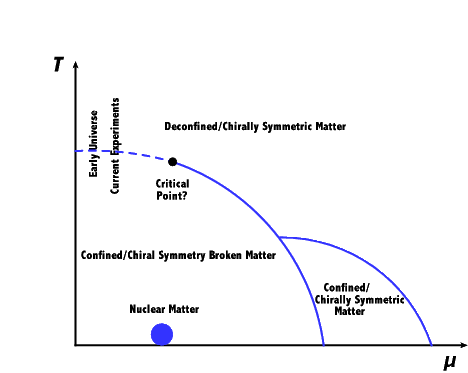
\includegraphics[width=5.5in]{figures/1742-6596-761-1-012066.png}\\
  \caption{Schematic of the QCD phase diagram \cite{1742-6596-761-1-012066}.}\label{fig:PhaseDiagram}
\end{figure}

The existence and properties of the QGP in the aftermath of high-energy heavy-ion collisions can be probed using different techniques relevant to several theoretical characteristics of the phase. For instance, the interacting nuclei  carry no net strangeness before colliding, and so a post-collision observation of strange and multi-strange particles can be a signal for an antecedent existence of deconfined quarks and gluons \cite{1742-6596-455-1-012005}. This signal, when complemented with an observation of the suppression???????or enhancement of strange particles production, provides a strong hint of the formation of QGP. This can be further complemented with the estimate of the energy density and the temperature attained after the collision.

Analyses of experimental results have thus far provided signatures of the formation of matter with partonic degrees of freedom at the early stages of the collisions. Such signatures include suppression of high monentum hadrons, known as jet quenching, because the QGP is nearly opaque to colored probes, and large azimuthal anisotropies, indicating that the medium is a liquid of quarks and gluons \cite{PhysRevC.96.044904}?????. Experiments also reveal the initial energy density of this matter to be about two orders of magnitude larger than that of low energy nuclear matter -- comfortably more than the deconfinement phase transition critical density predicted by lattice QCD \cite{2005PrPNP..54..443J}.

The state of the colliding nuclei before the collision at LHC and top RHIC energies has indications of being a Color Glass Condensate -- strongly interacting, weakly coupled highly coherent gluonic matter \cite{1742-6596-458-1-012024}. The characteristics of the initial states of these nuclei affect the partonic distributions within the nuclei and ultimately the products of the collision. The collision products are also affected by variables such as the initial energy and entropy densities of the partonic matter \cite{2005PrPNP..54..443J}.

Different observables can be used to study different aspects of heavy ion collisions. The charged particle multiplicity, $\langle N_{ch} \rangle$, is a global variable that relates to the entropy production during the collision (analysis note). The transverse energy, $E_{T}$, a global variable related to $\langle N_{ch} \rangle$, provides information about the conversion of the initial beam-direction kinetic energy into energy flowing in the transverse direction after the collision. Together, the studies of the fluctuation of the $\langle N_{ch} \rangle$ and the $E_{T}$ pseudorapidity [footnote] density with respect to the beam energy and the collision centrality [footnote] help probe the characteristics of the initial conditions at the time of the collision. One can study, for instance, the distinctions between models based on quark participants against those based on nucleon participants [analysis note]. These quantities can also lead to the rough estimate of the initial energy density through the use of the Bjorken formula \cite{2012ARNPS..62..361M}:
%\ref{eqn:Bjorken}
\begin{equation}\label{eqn:Bjorken}
\epsilon \geq \frac{\frac{dE_{T}}{d\eta}}{\tau_{0}\pi R^{2}} = \frac{3}{2}\langle \frac{E_{T}}{N} \rangle \frac{\frac{dN_{ch}}{d\eta}}{\tau_{0}\pi R^{2}}
\end{equation}

The transverse energy and the charged particle pseudorapidity densities have conventionally been calculated by using the transverse energy measurements obtained from calorimeters. This thesis details the use of particle spectra, reported as $\frac{d^{2}N}{dydp_{T}}$, from Au+Au collisions at RHIC to calculate the same global variables and serve as a method to cross check the ones involving calorimeters.

The organization of the thesis is as follows. Chapter II contains brief descriptions of different conventional methods used to estimate $E_{T}$ as well as an elaboration of the method specific to this thesis.
